\section{Rings} 

  \begin{definition}[Ring]
    A \textbf{ring} is a set $(R, +, \times)$ equipped with two operations, called addition and multiplication. It has properties: 
    \begin{enumerate}
      \item $R$ is an abelian group with respect to $+$, where we denote the additive identity as $0$ and the additive inverse of $x$ as $-x$. 
      \item $R$ is a monoid with respect to $\times$, where we denote the multiplicative identity as $1$, also known as the \textbf{unity}. 
      \item $\times$ is both left and right distributive with respect to addition $+$
      \begin{align}
        a \times (b + c) & = a\times b + a\times c \\ 
        (a + b) \times c & = a\times c + b\times c 
      \end{align}
      for all $a, b, c \in \mathbb{R}$. 
    \end{enumerate} 
    If $\times$ is associative, $R$ is called an \textbf{associative ring}, and if $\times$ is commutative, $R$ is called a \textbf{commutative ring}. 
  \end{definition}

  In fact, in some cases the existence of the multiplicative identity is not even assumed, though we will do it here.\footnote{If a multiplicative identity is not assumed, then this is called an \textit{rng}, or a \textit{rung}.}

  \begin{lemma} 
    Additive inverses are unique and $-1 \times a$ is the additive inverse of $a$. 
  \end{lemma}
  \begin{proof}
    We can see that 
    \begin{align}
      -1 + 1 = 0 & \implies (-1 + 1) \times a = 0 \times a \\
                 & \implies -1 \times a + 1 \times a = 0 \\
                 & \implies -1 \times a + a = 0 
    \end{align}
    and therefore by definition $-1 \times a$ must be the additive inverse. 
  \end{proof} 

  \begin{definition}[Characteristic Number]
    The \textbf{characteristic} of ring $R$, denoted char$(R)$, is the smallest number of times one must successively add the multiplicative identity $1$ to get the additive identity $0$. 
    \begin{equation}
      1 + 1 + ... + 1 = 0 
    \end{equation}
    If no such number $n$ exists, then char$(R) = 0$. 
  \end{definition}

  \begin{theorem}[Freshman's Dream]
    Given a field $F$ with char$(F) = p$, 
    \begin{equation}
      (a + b)^p = a^p + b^p
    \end{equation}
  \end{theorem}
  \begin{proof}
    We have 
    \begin{equation}
      (a + b)^p = \sum_{k = 0}^p \binom{p}{k} a^{p-k} b^{k}
    \end{equation}
    It is clear that 
    \begin{equation}
      \binom{p}{k} = \frac{p (p-1) ... (p - k+1)}{k!}
    \end{equation}
    is divisible by $p$ for all $k \neq 0, p$, so all the middle terms must cancel out to $0$. 
  \end{proof}


  Note that we do not assume that there exists multiplicative inverses in a ring. However, there may be some elements for which multiplicative inverses do exist, i.e. $a, b \in R$ where $ab = 1$.  

  \begin{definition}[Unit]
    A \textbf{unit} of a ring $R$ is an element $u \in R$ that has a multiplicative inverse in $R$. That is, there exists a $v \in R$ s.t. $uv = vu = 1$. 
  \end{definition}

  The next property that we would like to talk about is a zero divisor, which is the property that nonzero $a, b \in R$ satisfy $ab = 0$. 

  \begin{definition}[Left, Right Zero Divisor]
    An element $a$ of a ring $R$ is called a \textbf{left zero divisor} if there exists a nonzero $x$ such that $a x = 0$ and a \textbf{right zero divisor} if there exists a nonzero $x$ such that $x a = 0$. 
  \end{definition} 

  Another property that we would desire is some sort of decomposition of ring elements as other ring elements. 

  \begin{definition}[Left, Right Divisor]
    Let $a, b \in R$ a ring. 
    \begin{enumerate}
      \item If there exists an element $x \in R$ with $ax = b$, we say $a$ is a \textbf{left divisor} of $b$. 

      \item If there exists an element $y \in R$ with $ya = b$, we say $a$ is a \textbf{right divisor} of $b$. 

      \item We say $a$ is a \textbf{two-sided divisor} if it is both a left divisor and a right divisor of $b$. Note that the $x$ and $y$ are not required to be equal. 
    \end{enumerate}
  \end{definition}

  It turns out that the existence of units and zero divisors classify rings into subcategories, which we will elaborate on. That is, we will start with the most general theory on rings, and then shrink down into subcategories of rings. 

  \begin{figure}[H]
    \centering 
    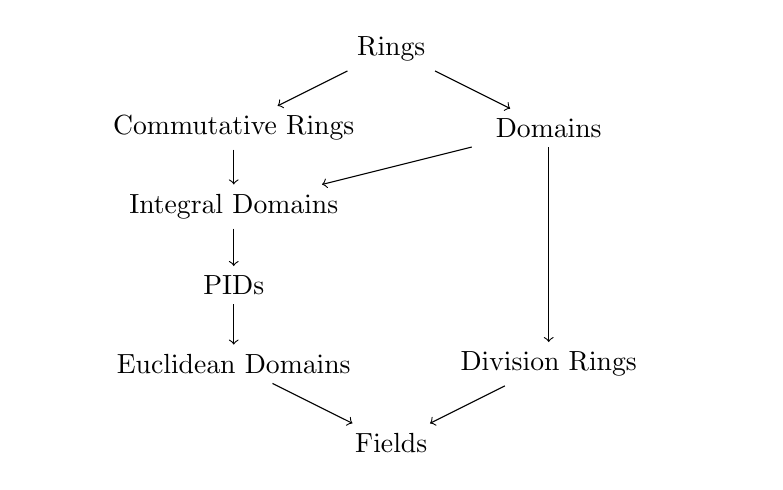
\begin{tikzpicture}[
        node distance=2cm,
        box/.style={
            text width=5cm,
            align=center
        }
    ]
        % Nodes for ring types
        \node[box] (rings) at (0,0) {Rings};
        \node[box] (comm) at (-2,-1) {Commutative Rings};
        \node[box] (domains) at (2,-1) {Domains};
        \node[box] (int) at (-2,-2) {Integral Domains};
        \node[box] (divring) at (2,-4) {Division Rings};
        \node[box] (pid) at (-2,-3) {PIDs};
        \node[box] (euc) at (-2,-4) {Euclidean Domains};
        \node[box] (fields) at (0,-5) {Fields};
        
        % Left path arrows
        \draw[->] (rings) -- (comm);
        \draw[->] (comm) -- (int);
        \draw[->] (int) -- (pid);
        \draw[->] (pid) -- (euc);
        \draw[->] (euc) -- (fields);
        \draw[->] (divring) -- (fields);
        
        % Right path arrows
        \draw[->] (rings) -- (domains);
        \draw[->] (domains) -- (int);
        \draw[->] (domains) -- (divring);
    \end{tikzpicture}
    \caption{Basic hierarchy of rings.} 
    \label{fig:ring_hierarchy}
  \end{figure} 

  \begin{example}[Integers, Rationals, Reals, Complexes]
    The fields $\mathbb{Z}, \mathbb{Q}$, $\mathbb{R}$, and $\mathbb{C}$ are rings with:
    \begin{enumerate}
      \item Sets: 
        \begin{itemize}
          \item $\mathbb{Q}$: rational numbers $\{\frac{a}{b} : a,b \in \mathbb{Z}, b \neq 0\}$
          \item $\mathbb{R}$: real numbers
          \item $\mathbb{C}$: complex numbers $\{a + bi : a,b \in \mathbb{R}\}$
        \end{itemize}
      \item Standard addition and multiplication
      \item Additive identity 0
      \item Multiplicative identity 1
    \end{enumerate}
    These form commutative rings with unity where every non-zero element has a multiplicative inverse.
  \end{example}

  \begin{example}[Continuous Functions]
    The set of all continuous functions $f: \mathbb{R} \rightarrow \mathbb{R}$ is a ring under point-wise addition and multiplication. 
  \end{example}

  \begin{example}[Matrices]
    The ring $M_n(R)$ of $n \times n$ matrices over a ring $R$ consists of:
    \begin{enumerate}
      \item $n \times n$ arrays of elements from $R$
      \item Matrix addition (entry-wise):
      \begin{equation}
        (A + B)_{ij} = A_{ij} + B_{ij}
      \end{equation}
      \item Matrix multiplication:
      \begin{equation}
        (AB)_{ij} = \sum_{k=1}^n A_{ik}B_{kj}
      \end{equation}
      \item Zero matrix as additive identity
      \item Identity matrix $I_n$ as multiplicative identity
    \end{enumerate}
    This forms a non-commutative ring for $n > 1$, even when $R$ is commutative.
  \end{example}

  \begin{example}[Power Set]
    Given a set $X$, let $2^X$ be its power set, that is the set of all subsets of $X$. Then, $2^X$ is a commutative associative ring with respect to the operations of symmetric difference (i.e. the set of elements which is in exactly one of the sets) 
    \begin{equation}
      M \bigtriangleup N \equiv (M \setminus N) \cup (N \setminus M)
    \end{equation}
    and intersection $\cap$, taken for addition an multiplication, respectively. We will not prove all of the axioms of the ring, but we can state some important facts about this structure. The additive identity is $\emptyset$ and the multiplicative identity is $X$. Finally, it is clear that 
    \begin{align*}
      & M \bigtriangleup N \equiv (M \setminus N) \cup (N \setminus M) \equiv N \bigtriangleup M \\
      & M \cap N = N \cap M \\
      & M \cap N \cap P = (M \cap N) \cap P = M \cap (N \cap P)
    \end{align*}
  \end{example}

\subsection{Ring Homomorphisms and Characteristics}

  So far, we have talked about many properties of rings but have not thoroughly gone over their classification. This is what we will do in this section, just like how we have classified groups. It turns out that classifying rings is significantly harder to do so, so we will talk about some low-order finite rings and provide some examples of isomorphisms between more complex rings. Recall that in point set topology, given a topological space $(X, \mathscr{T})$ and its quotient space, if we can construct a map from $X$ to a cleverly chosen space $Z$ that agrees with the quotient, then this induces a homeomorphism $X \cong Z$. 

  \begin{definition}[Ring Homomorphism, Isomorphism]
    A \textbf{ring homomorphism} $f: R \rightarrow S$ is a function that satisfies for all $a, b \in R$
    \begin{enumerate}
      \item $f(a + b) = f(a) + f(b)$
      \item $f(ab) = f(a) f(b)$ 
      \item $f(1_R) = 1_S$
    \end{enumerate}
    for all $a, b \in R$.\footnote{Note that the first is equivalent to it being a group homomorphism between $(R, +)$ and $(S, +)$. The second property may look like it is a group homomorphism between $(R, \times)$ and $(S, \times)$, but remember that neither are groups and it just states that closure distributes. Combined with the fact that the multiplicative identity matches, $f$ is really a homomorphism of \textit{monoids}. } If $f$ is a bijective ring homomorphism, it is called a \textbf{ring isomorphism}. 
  \end{definition} 

  \begin{definition}[Kernel]
    The \textbf{kernel} of a ring homomorphism $f: R \rightarrow S$ is the preimage of $0 \in S$.\footnote{Note that this is the additive identity, not the multiplicative identity. We must specify which identity, unlike a group which has just one identity.}
  \end{definition}

  \begin{lemma}[Properties of Ring Homomorphisms]
    It immediately follows that if $f: R \rightarrow S$ is a ring homomorphism, then 
    \begin{enumerate}
      \item $f(0) = 0$ 
      \item $\Im(f)$ is a subring of $S$. 
      \item A ring homomorphism is injective if and only if $\ker{f} = \langle 0 \rangle $.  
    \end{enumerate}
    Furthermore, if $f$ is a ring isomorphism, then 
    \begin{enumerate}
      \item $f^{-1}$ is a ring isomorphism. 
    \end{enumerate}
  \end{lemma}

  \begin{theorem}[Compositions of Ring Homomorphisms]
    Compositions of ring homomorphisms are ring homomorphisms. 
  \end{theorem} 

\subsection{Commutative Rings} 

  Note that for commutative rings, distinguishing left and right divisors are meaningless, and so we can talk about just \textit{divisors}. 

  \begin{lemma}[Left=Right Divisors]
    In a commutative ring $R$, $a$ is a left divisor of $b$ iff $a$ is a right divisor of $b$. In this case, we just say that $a$ is a \textbf{divisor} of $b$, written $a | b$. 
  \end{lemma}
  \begin{proof}
    $a$ is a right divisor of $b \iff \exists x (xa = b) \iff \exists x (ax = b) \iff a$ is a left divisor. 
  \end{proof} 

  \begin{definition}[Prime and Compositive Elements]
    In a commutative ring $R$, an element $p \in R$ is said to be \textbf{prime} if it is not $0$, not a unit, and has only divisors $1$ and $p$. 
  \end{definition}

  \begin{lemma}[Euclid]
    If $p$ is prime, then $p|ab \implies p|a$ or $p|b$.  
  \end{lemma}

  \begin{lemma} 
    Let $R$ be a commutative ring and $a, b, d \in R$. If $d|a$ and $d|b$, then $d | (ma + nb)$ for any $m, n \in R$. 
  \end{lemma} 

  \begin{definition}[Greatest Common Divisor]
    The \textbf{greatest common divisor} of elements $a$ and $b$, denoted $\gcd(a, b)$ of an commutative ring $R$ is a common divisor of $a$ and $b$ divisible by all their common divisors. That is, it is the element $d \in R$ satisfying 
    \begin{enumerate}
      \item $d \mid a$ and $d \mid b$ 
      \item if $k \mid a$ and $k \mid b$, then $k \mid d$. 
    \end{enumerate}
    If $\mathrm{gcd}(a, b) = 1$, then $a$ and $b$ are said to be \textbf{relatively prime}. 
  \end{definition} 

  Note that in an arbitrary commutative ring, the gcd of two elements always exists since we can at least identify $1$, but there may not be a \textit{unique} gcd. 

\subsection{Domains}

  We can see that domains behave similarly to the integers, but with the missing property that $\times$ is commutative. This motivates the following definition of an integral domain, which can be seen as a generalization of the integers. 

  \begin{definition}[Domain]
    A ring $R$ with no zero divisors for every element is called a \textbf{domain}. An \textbf{integral domain} is a commutative domain $R$.\footnote{Almost always, we work with integral domains so we will default to this.} 
  \end{definition} 

  \begin{example}[Domains vs Integral Domains]
    We show some examples of integral domains. 
    \begin{enumerate}
      \item The ring $\mathbb{Z}$ of integers. 
      \item The field $\mathbb{R}$. 
      \item The ring $\mathbb{Z}[x]$ of polynomials of one variable with integer coefficients. 
    \end{enumerate}
    We show examples of domains that are not integral domains. 
    \begin{enumerate}
      \item Quaternions $\mathbb{H}$ are not commutative but are a domain. 
    \end{enumerate}
  \end{example} 

  \begin{theorem}[Fields are Integral Domains]
    Every field is an integral domain. 
  \end{theorem}
  \begin{proof}
    
  \end{proof}

  \begin{theorem}[Polynomial Integral Domains]
    Rings of polynomials are an integral domain if the coefficients come from an integral domain. 
  \end{theorem}
  \begin{proof}
    
  \end{proof} 

  Factorization of polynomials over $\mathbb{C}$ into linear factors and polynomials over $\mathbb{R}$ into linear and quadratic factors is similar to the factoring of the integers to prime numbers. In fact, such a factorization exists for polynomials over any field $F$, but their factors can be of any degree. Moreover, there exists no general solution for the factoring of polynomials over any field. 

  \begin{example}
    $\mathbb{Z}$ and $F[x]$ over field $F$ are integral domains. Any field $F$ is also an integral domain. 
  \end{example}

  \begin{example}
    The quotient ring $\mathbb{Z}_n$ is not an integral domain when $n$ is composite. 
  \end{example}

  \begin{example}
    A product of two nonzero commutative rings with unity $R \times S$ is not an integral domain since $(1,0) \cdot (0, 1) = (0, 0) \in R \times S$. 
  \end{example}

  \begin{example}
    The ring of $n \times n$ matrices over any nonzero ring when $ n \geq 2$ is not an integral domain. Given matrices $A, B$, if the image of $B$ is in the kernel of $A$, then $A B = 0$.
  \end{example}

  \begin{example}
    The ring of continuous functions on the interval is not an integral domain. To see why, notice that given the piecewise functions 
    \begin{equation}
      f (x) = \begin{cases}
      1 - 2x & x \in [0, \frac{1}{2}] \\
      0 & x \in [\frac{1}{2}, 1] 
      \end{cases}, \; \;\;g (x) = \begin{cases}
      0 & x \in [0, \frac{1}{2}] \\
      2x - 1 & x \in [\frac{1}{2}, 1] 
      \end{cases}
    \end{equation}
    $f, g \neq 0$, but $f g = g f = 0$. 
  \end{example}

  \begin{theorem}
    An integral domain is a ring that is isomorphic to a subring of a field. 
  \end{theorem}

  \begin{theorem}
    The characteristic of an integral domain is either $0$ or a prime number. 
  \end{theorem}

  \begin{definition}[Regular Elements]
     An element $r$ of a ring $R$ is \textbf{regular} if the mapping 
     \begin{equation}
       \rho: R \longrightarrow R, \qquad x \mapsto x r
     \end{equation}
    is injective for all $x \in R$. 
  \end{definition}

  \begin{theorem}
    An integral domain is a commutative associative ring where every element is regular. 
  \end{theorem} 

  While we have shown that gcd's exist in commutative rings, we can say a bit more when working in Euclidean domains. 

  \begin{definition}[Associate Elements]
    Elements $a$ and $b$ are \textbf{associated}, denoted $a \sim b$ if either of the following equivalent conditions holds
    \begin{enumerate}
        \item $a | b \text{ and } b | a$
        \item $a = c b, \text{ where } c$ is invertible
    \end{enumerate}
    The two conditions are equivalent because $c$ and $c^{-1}$ are both in $A$. 
  \end{definition} 

  \begin{theorem}[GCD's in a Euclidean Domain]
    Any two distinct gcd's of $a, b$ in a Euclidean domain must be associate elements. 
  \end{theorem}

\subsection{Ideals}

  Now assuming that $R$ and $S$ are commutative rings, let's consider a special sort of subset of a commutative ring. Consider the kernel of the ring homomorphism. We can see that if $a, b \in \ker(f)$, then $f(a + b) = f(a) + f(b) = 0 + 0 = 0$, and so $\ker(f)$ is closed under addition. Furthermore, $a \in \ker(f)$ and \textit{any} $b \in R$ gives $f(ab) = f(a) f(b) = 0 f(b) = 0$, and so multiplying any element in the kernel by an arbitrary element in the rings keeps it in the kernel. We would like to generalize these properties into an \textit{ideal}. 

  \begin{definition}[Ideals]
    For a commutative ring $(R,+, \times)$, a \textbf{two-sided ideal}---or \textbf{ideal}---is a subset $I \subset R$ satisfying 
    \begin{enumerate}
      \item $a, b \in I \implies a + b \in I$. 
      \item $a \in I, r \in R \implies ra = ar \in I$.
    \end{enumerate}
    If $R$ is not necessarily commutative, then we $ra \neq ar$ in general, so we may distinguish between left and right ideals. 
  \end{definition}

  Let's try to elaborate more on this interpretation by introducing immediate consequences. 

  \begin{lemma}[Ideals are Groups Under $+$]
    Given a commutative ring $R$ and ideal $I \subset R$, $(I, +)$ is an abelian group. 
  \end{lemma}

  Therefore, we can see that it is an abelian group under $+$ and closed under $\times$. However, it is not guaranteed to have a multiplicative identity, which is why we can interpret $I$ as a ring without a multiplicative identity, also known as a \textit{rung}. 

  \begin{example}[Multiples of Elements Are an Ideal]
    We give 2 ideals: 
    \begin{enumerate}
      \item The set of even integers $2 \mathbb{Z}$ is an ideal in the ring $\mathbb{Z}$, since the sum of any even integers is even and the product of any even integer with an integer is an even integer. However, the odd integers do not form an ideal. 
      \item The set of all polynomials with real coefficients which are divisible by the polynomial $x^2 + 1$ is an ideal in the ring of all polynomials. 
    \end{enumerate}
  \end{example}

  Given these two examples, we can think of an ideal consisting of all multiples of a specific element $a$ that \textit{generates} the ideal. 

  \begin{definition}[Generators of Ideals]
    Given a commutative ring $R$, the \textbf{ideal generated by $a \in R$} is denoted 
    \begin{equation}
      \langle a \rangle \coloneqq \{r a \mid r \in R\}
    \end{equation}
    and more generally, we may have multiple generating elements. 
    \begin{equation}
      \langle a_1, \ldots, a_n \rangle \coloneqq \{ r_1 a_1 + \ldots r_n a_n \mid r_1, \ldots, r_n \in R \}
    \end{equation}
  \end{definition}

  Therefore, the ideals considered above can be written $\langle 2 \rangle \subset \mathbb{Z}$ and $\langle x - 2 \rangle \subset \mathbb{Q}[x]$. However, it may be the case that two elements generate the same ideal in a non-Euclidean domain, but constructing such an example is a bit challenging.   

  \begin{example}[Matrix with Last Row of Zeros]
    The set of all $n \times n$ matrices whose last row is zero forms a right ideal in the ring of all $n \times n$ matrices. However, it is not a left ideal.

    The set of all $n\times n$ matrices whose last column is zero is a left ideal, but not a right ideal. 
  \end{example}

  \begin{theorem}[Ideals of Fields]
    The only ideals that exist in a field $\mathbb{F}$ is $\{0\}$ and $\mathbb{F}$ itself. 
  \end{theorem}
  \begin{proof}
    Given a nonzero element $x \in \mathbb{F}$, every element of $\mathbb{F}$ can be expressed in the form of $a x$ or $x a$ for some $a \in \mathbb{F}$. 
  \end{proof}

\subsection{Quotient Rings}

  What is nice about ideals is that they induce an equivalence relation defined on a ring, which reminds you of working in modulos on the integers. 

  \begin{theorem}[Equivalence Relation Induced by an Ideal]
    Given a commutative ring $R$ and an ideal $I \subset R$, we say that two elements $a, b \in R$ are equivalent $\pmod{I}$, written $a \equiv b \pmod{I}$ iff $a - b \in I$. We claim two things: 
    \begin{enumerate}
      \item $\equiv$ is indeed an equivalence relation. 
      \item Given that $a \equiv a^\prime \pmod{I}$ and $b = b^\prime \pmod{I}$, 
        \begin{equation}
          a + b \equiv a^\prime + b^\prime \pmod{I}, \qquad ab \equiv a^\prime b^\prime \pmod{I}
        \end{equation}
    \end{enumerate}
  \end{theorem}
  \begin{proof}
    We first prove that $\equiv$ is indeed an equivalence relation. 
    \begin{enumerate}
      \item \textit{Reflexive}. $a \equiv a \pmod{I}$ is trivial since $a - a = 0 \in I$. 
      \item \textit{Transitive}. If $a \equiv b$. 
    \end{enumerate}
  \end{proof} 

  This quotient space maintains a lot of nice properties of the algebraic operations, and so we can form a new ring structure with this quotient space.  

  \begin{definition}[Quotient Rings, Rings of Residue Class]
    The quotient space $R/I$ induced by the mapping $a \mapsto [a]$ is indeed a commutative ring, called the \textbf{quotient ring}, with addition and multiplication defined 
    \begin{equation}
      [a] + [b] \coloneqq [a + b], \qquad [ab] \coloneqq [a] \, [b]
    \end{equation}
  \end{definition}
  \begin{proof}
    Note that the properties of the operation in $\frac{M}{R}$ inherits all the properties of the addition operation on $M$ that are expressed in the form of identities and inverses, along with the existence of the zero identity. 
    \begin{align*}
      0 \in M & \implies [0] \text{ is the additive identity in } \frac{M}{R} \\
      a + (-a) = 0 & \implies [a] + [-a] = [0] \\
      1 \in M & \implies [1] \text{ is the multiplicative identity in } \frac{M}{R}
    \end{align*}
  \end{proof} 

  \begin{example}[Quotient Rings of Integers]
    The quotient set $\mathbb{Z}/\langle n \rangle$ by the relation of congruence modulo $n$ is denoted $\mathbb{Z}_{n}$. 
    \begin{equation}
      \mathbb{Z}_{n} = \{ [0]_{n}, [1]_{n}, \ldots, [n-1]_{n} \}
    \end{equation}
    We list some quotient rings of the integers.  
    \begin{enumerate}
      \item In $\mathbb{Z}_{5} = \mathbb{Z}/\langle 5 \rangle$, the elements $[2]$ and $[3]$ are multiplicative inverses of each other since $[2] [3] = [6] = [1]$, and $[4]$ is its own inverse since $[4] [4] = [16] = [1]$. The addition and multiplication tables for $\mathbb{Z}_5$ is shown below. 
      \item Consider the ideal $I = \langle 2 \rangle \subset \mathbb{Z}_6$. We have $0 \equiv 2 \equiv 4 \pmod{I}$ and $1 \equiv 3 \equiv 5 \pmod{I}$, and so the quotient ring $\mathbb{Z}_6 / I$ consists of the two equivalence classes $[0]$ and $[1]$. 
    \end{enumerate}
  \end{example}

  \begin{example}[Quotient Rings of Polynomials]
    We list some quotient rings of the integers.  
    \begin{enumerate}
      \item Consider $\mathbb{Q}[x] / \langle x^2 - 2 \rangle$. We can see that any polynomial $f \in \mathbb{Q}[x]$ is equivalent $\pmod{I}$ to a linear polynomial, since $x^2 \equiv 2$. Alternatively we can apply the division algorithm to replace $f(x)$ by its remainder upon division by $x^2 - 2$, and thus in the quotient ring, $[x]$ plays the role of $\sqrt{2}$, which may indicate that $\mathbb{Q}[x] / \langle x^2 - 2 \rangle = \mathbb{Q}[\sqrt{2}]$. 
      \item Consider $\mathbb{Z}_2 [x]/ \langle x^2 + x + 1 \rangle$. As in the previous example, any polynomial in $\mathbb{Z}_2[x]$ is equivalent to a linear polynomial since $x^2 \equiv x + 1 \pmod{I}$. Therefore the elements of the quotient ring are $[0], [1], [x], [x+1]$ with the addition and multiplication tables. 

      \begin{figure}[H]
        \centering
        \begin{subfigure}[b]{0.48\textwidth}
          \centering
          \begin{tabular}{c|cccc}
            $+$ & $0$ & $1$ & $x$ & $x + 1$ \\
            \hline
            $0$ & $0$ & $1$ & $x$ & $x + 1$ \\
            $1$ & $1$ & $0$ & $x + 1$ & $x$ \\
            $x$ & $x$ & $x + 1$ & $0$ & $1$ \\
            $x + 1$ & $x + 1$ & $x$ & $1$ & $0$ \\
          \end{tabular}
          \caption{}
        \end{subfigure}
        \hfill 
        \begin{subfigure}[b]{0.48\textwidth}
          \centering
          \begin{tabular}{c|cccc}
            $\cdot$ & $0$ & $1$ & $x$ & $x + 1$ \\
            \hline
            $0$ & $0$ & $0$ & $0$ & $0$ \\
            $1$ & $0$ & $1$ & $x$ & $x + 1$ \\
            $x$ & $0$ & $x$ & $x + 1$ & $1$ \\
            $x + 1$ & $0$ & $x + 1$ & $1$ & $x$ \\
          \end{tabular}
          \caption{}
        \end{subfigure}
        \label{fig:boolean-algebra-tables}
      \end{figure}
    \end{enumerate}
  \end{example}

  Note that just like how quotient topologies do not preserve topological properties, as shown \hyperref[pst-quotient_trivial]{here} and \hyperref[pst-quotient_hausdorff]{here}, quotient rings inherit some---but not all---algebraic properties. 

  \begin{theorem}[Quotient Inherits Commutativity]
    Let $R$ be a commutative ring and $I \subsetneq R$ be an ideal. Then $R/I$ is a commutative ring. 
  \end{theorem}

  \begin{example}[Quotient Does Not Inherit Integral Domain Property]
    $\mathbb{Z}$ is an integral domain, but $\mathbb{Z}/\langle 6 \rangle$ is not since $[2] \times [3] = [0]$. 
  \end{example}


  The ring $\mathbb{Z}_n$ has all the properties of a field except the property of having inverses for all of its nonzero elements. This leads to the following theorem. 

  \begin{theorem}[Integer Quotient Rings as Finite Fields]
    The ring $\mathbb{Z}_{n}$ is a field if and only if $n$ is a prime number. 
  \end{theorem}
  \begin{proof}
    $(\rightarrow)$ Assume that $n$ is composite $\implies n = k l$ for $k, n \in \mathbb{N} \implies k, n \neq 0$, but 
    \begin{equation}
      [k]_n [l]_n = [k l]_n = [n]_n = 0
    \end{equation}
    meaning that $\mathbb{Z}_n$ contains $0$ divisors and is not a field. The contrapositive of this states $(\rightarrow)$. \\
    $(\leftarrow)$ Given that $n$ is prime, let $[a]_n \neq 0$, i.e. $[a]_n \neq [0]_n, [1]_n$. The set of $n$ elements 
    \begin{equation}
      [0]_n, [a]_n, [2a]_n, ..., [(n-1)a]_n
    \end{equation}
    are all distinct. Indeed, if $[k a]_n = [l a]_n$, then $[(k-l) a]_n = 0 \implies n = (k-l) a \iff n$ is not prime. Since the elements are distinct, exactly one of them must be $[1]_n$, say $[p a]_n \implies$ the inverse $[p]_n$ exists. 
  \end{proof}

  \begin{corollary}[Invertibility in $\mathbb{Z}_n$]
    For any $n$, $[k]_n$ is invertible in the ring $\mathbb{Z}_n$ if and only if $n$ and $k$ are relatively prime. 
  \end{corollary} 

  \begin{theorem}[Wilson's Theorem]
    Let $n$ be a prime number. Then 
    \begin{equation}
      (n-1)! \equiv -1 \pmod{n}
    \end{equation}
  \end{theorem}

\subsection{Homomorphism and Isomorphism Theorems}

  \begin{theorem}[Fundamental Ring Homomorphism Theorem]
    Let $R$ and $S$ be commutative rings, and suppose $f: R \rightarrow S$ be a surjective ring homomorphism. Then this induces a ring isomorphism
    \begin{equation}
      R /\ker{f} \simeq S
    \end{equation} 
    satisfying $\phi = \bar{\phi} \circ \pi$. 

    \begin{figure}[H]
      \centering 
      \begin{tikzcd}
        R \arrow[r, "\phi"] \arrow[d, "\pi"] & S \\
        R/\ker(\phi) \arrow[ru, "\bar{\phi}"] &  
      \end{tikzcd}
      \caption{The theorem states that the following diagram commutes. } 
      \label{fig:fund_ring_homo_theorem}
    \end{figure}
  \end{theorem}
  \begin{proof}
    
  \end{proof} 

\subsection{Unique Factorization Domain}

\subsection{Principal Ideal Domains}

  A good intuition to have about ideals is that they are the set of multiples of a certain element. However, this may not be true for ideals in general, but if this intuition is true, then we call this a \textit{principal ideal}. 

  \begin{definition}[Principal Ideals]
    Given commutative ring $R$ and $I \subset R$, if $I = \langle a \rangle$ for some $a \in R$---i.e. it is generated by a single element---$I$ is called a \textbf{principal ideal}. 
  \end{definition}

  \begin{definition}[Principal Ideal Domain]
    A \textbf{principal ideal domain}, also called a \textbf{PID}, is an integral domain in which every ideal is principal. 
  \end{definition}

  More generally, a \textbf{principal ideal ring} is a nonzero commutative ring in which every ideal is principal (i.e. can be generated by a single element). The distinction is that a principal ideal ring may have zero divisors whereas a principal ideal domain cannot. Principal ideal domains are thus mathematical objects that behave somewhat like the integers. That is, 
  \begin{enumerate}
    \item Any element of a PID has a unique decomposition into prime elements. 
    \item Any two elements of a PID have a greatest common divisor. 
    \item If $x$ and $y$ are elements of a PID without common divisors, then every element of the PID can be written in the form 
      \begin{equation}
        a x + b y
      \end{equation}
  \end{enumerate}

  We now introduce some examples of PIDs, which are not as trivial and should be introduced as theorems. 

  \begin{theorem}[Integers and Polynomials over Fields are PIDs]
    The following are all examples of principal ideal domains. 
    \begin{enumerate}
      \item Any field $\mathbb{F}$. 
      \item The ring of integers $\mathbb{Z}$. 
      \item $\mathbb{F}[x]$, rings of polynomials in one variable with coefficients in a field $\mathbb{F}$. 
    \end{enumerate}
  \end{theorem}
  \begin{proof}
    Listed. 
    \begin{enumerate}
      \item It is quite easy to see that a field $\mathbb{F}$ is a PID since the only two possible ideals are $\{0\}$ and $\mathbb{F}$, both of which are principal. 
      \item If $I \subset \mathbb{Z}$ is an ideal, then if $I = \langle 0 \rangle$, then we're done. Otherwise, let $a \in I$ be the smallest positive integer in $I$. It is clear that $\langle a \rangle \subset I$. Now given an element $b \in I$, by the Euclidean algorithm we have $b = aq + r$ with $r < a$. Since $a, b \in I$, it follows that $r \in I$. But since $0 \leq r < a$ and $a$ is the smallest positive integer, $r = 0$, and so $b = aq \implies b \in \langle a \rangle$. 
      \item The ring of polynomials $\mathbb{F}[x]$ is a PID since we can imagine a minimal polynomial $p$ in each ideal $I$. Every element in $I$ must be divisible by $p$, which means that the entire ideal $I$ can be generated by the minimal polynomial $p$, making $I$ principal.  
    \end{enumerate}
  \end{proof}

  \begin{corollary}[Ideals Generated by Primes]
    If $I \subsetneq \mathbb{Z}$ and a prime number $p \in I$, then $I = \langle p \rangle$. If $I \subset F[x]$ is an ideal and irreducible $f(x) \in I$, then $I = \langle f(x) \rangle$. 
  \end{corollary}
  \begin{proof}
    Listed. 
    \begin{enumerate}
      \item Since $\mathbb{Z}$ is a PID, $I = \langle a \rangle$ for some nonzero $a \in \mathbb{Z}$. We can assume $a$ is positive, and if $a = 1$, then $I = \mathbb{Z}$, which contradicts the $I$ is a proper subset. So $a \geq 2$. Now because $p \in I$, $p = ra$ for some $r \in \mathbb{Z}$, but since $p$ is prime, $r = 1, a = p$. 

      \item Since $F[x]$ is a PID and $I = \langle g(x) \rangle$ for some $g(x) \in F[x]$, let us take $f(x) \in I$. Then it must be true that $f(x) = g(x) h(x)$ for some $h(x) \in R$. However, This means that $\deg(g)$ or $\deg(h)$ must be $0$ since $f$ is irreducible. But if $g(x)$ was a constant, then $I = R$, so $g(x) = f(x)$. 
    \end{enumerate}
  \end{proof}

  \begin{corollary}[Kernel of Evaluation Homomorphism is Generated by Irreducible Factor]
    Suppose $f(x) \in F[x]$ is irreducible in $F[x]$, and $K \supset F$ is a field containing a root $\alpha$ of $f(x)$. Then the ideal of all polynomials in $F[x]$ vanishing at $\alpha$ is generated by $f(x)$. That is, given the evaluation homomorphism 
    \begin{equation}
      \ev_\alpha: F[x] \rightarrow K
    \end{equation}
    we claim $\ker(\ev_\alpha) = \langle f(x) \rangle$. 
  \end{corollary}
  \begin{proof}
    This is an immediate consequence of the previous corollary. 
  \end{proof}

  The great thing about PIDs is that they unlock a lot of the familiar properties that we see in the integers. In fact, pretty much everything holds except for the existence of Euclidean algorithm for factorization. 

  \begin{theorem}[Greatest Common Divisor]
    Given $a, b \in R$ a PID, $\gcd(a, b)$ is unique. 
  \end{theorem}

  \begin{theorem}[Unique Factorization Theorem]
    Every element $x \in R$ of a PID can be uniquely factored (up to permutations and units) into irreducible elements in $R$. 
  \end{theorem}

  Bezout's does not hold in integral domains in general. 

  \begin{theorem}[Bezout's Theorem]
    Given that one divides (with remainder) polynomial $f$ by $g = x - c$, let the remainder be $r \in F$. That is, 
    \begin{equation}
      f(x) = (x-c) q(x) + r, \; r \in F
    \end{equation}
    This implies that the remainder equals the value of $f$ at point $c$. That is, 
    \begin{equation}
      f(c) = r
    \end{equation}
    Note that a corollary of this is the single factorization theorem, but the single factorization holds for commutative rings in general. 
  \end{theorem} 

\subsection{Euclidean Domains}

  \begin{definition}[Euclidean Domain]
    Let $R$ be an integral domain which is not a field. $R$ is \textbf{Euclidean domain} if 
    \begin{enumerate}
      \item there exists a \textit{norm} $|\cdot|: R \setminus \mathbb{R}_0^+$, and  
      \item there exists a well-defined function, called \textbf{Euclidean division} $\mathcal{D}: R \times R \rightarrow R \times R$ that is defined 
      \begin{equation}
        \mathcal{D}(a, b) = (q, r) \text{ where } a = bq + r \text{ and } 0 \leq r < |b|
      \end{equation}
    \end{enumerate}
  \end{definition}

  The two prime examples are the integers and polynomials. 

  \begin{example}[Integers]
    $\mathbb{Z}$ is a Euclidean domain with Euclidean division, also called long division, defined 

    \begin{center}
      \intlongdivision{521}{13}
    \end{center}
  \end{example}

  \begin{theorem}[Polynomials are Euclidean Domains]
    Let $f(x), g(x) \in F[x]$ and $g(x) \neq 0$. Then, there exists polynomials $q(x), r(x)$ such that 
    \begin{equation}
      f(x) = q(x) g(x) + r(x), \qquad 0 \leq \deg(r) < \deg(g)
    \end{equation}
    where $\deg$ is the norm.
  \end{theorem}

  \begin{example}[Gaussian Integers]
    The subring of $\mathbb{C}$, defined
    \begin{equation}
      \mathbb{Z}[i] \equiv \{ a + b i \mid a, b \in \mathbb{Z} \}
    \end{equation}
    is a Euclidean integral domain with respect to the norm 
    \begin{equation}
      N(c) \equiv a^2 + b^2
    \end{equation}
    since $N(c d) = N(c) N(d)$ and the invertible elements of $\mathbb{Z}[i]$ are $\pm 1, \pm i$. 
  \end{example}

  \begin{example}[Dyadic Rationals]
    The ring of rational numbers of the form $2^{-n} m, \; n \in \mathbb{Z}_+, m \in \mathbb{Z}$, is a Euclidean domain. To define the norm, we can first assume that $m$ can be prime factorized into the form 
    \begin{equation}
      m = \pm \prod_{i} p_{i}^{k_i}, \; p \text{ prime}
    \end{equation}
    and the norm is defined 
    \begin{equation}
      N(\frac{m}{2^n}) \equiv 1 + \sum_i k_i
    \end{equation}
    We must further show that division with remainder is possible, but we will not show it here. 
  \end{example}

  \begin{theorem}[Chinese Remainder Theorem]
    
  \end{theorem}

\subsection{Division Rings}

  \begin{definition}[Division Ring]
    A \textbf{division ring}, also called a \textbf{skew field}, is an associative ring where every nonzero element is invertible with respect to $\times$.\footnote{Division rings differ from fields in that multiplication is not required to be commutative. }
  \end{definition}

  Let's establish the hierarchy. 

  \begin{lemma}[Division Rings are Domains]
    Every division ring $R$ is automatically a domain. 
  \end{lemma}
  \begin{proof}
    Every nonzero element is invertible. 
  \end{proof}

  \begin{example}[Invertible Matrices are a Division Ring]
    At first, a division ring may not seem different from a field. However, a classic example is the ring of invertible matrices, which is not necessarily commutative, but is a ring in which "division" can be done by right and left multiplication of a matrix inverse. 
    \begin{equation}
      a a^{-1} = a^{-1} a = I
    \end{equation}
    This implies that every element in the division ring commutes with the identity, but again commutativity does not necessarily hold for arbitrary elements $a, b$. 
  \end{example} 

\subsection{Fields}

  Our final structure is field, which are usually pretty tame compared to groups and rings. 

  \begin{definition}[Field]
    A \textbf{field} $(F, +, \times)$ is a commutative, associative ring where every nonzero element is a unit. 
  \end{definition}

  \begin{lemma}[Properties of Addition]
    The properties of addition hold in a field. 
    \begin{enumerate}
      \item If $x + y = x + z$, then $y = z$. 
      \item If $x + y = x$, then $y = 0$. 
      \item If $x + y = 0$, then $y = -x$. 
      \item $(-(-x)) = x$. 
    \end{enumerate}
  \end{lemma}
  \begin{proof}
    For the first, we have 
    \begin{align}
      x + y = x + z & \implies -x + (x + y) = -x + (x + z) && \tag{addition is a function} \\
                    & \implies (-x + x) + y = (-x + x) + z && \tag{$+$ is associative} \\
                    & \implies 0 + y = 0 + z && \tag{definition of additive inverse} \\
                    & \implies y = z && \tag{definition of identity}
    \end{align} 
    For the second, we can set $z = 0$ and apply the first property. For the third, we have 
    \begin{align}
      x + y = 0 & \implies -x + (x + y) = -x + 0 && \tag{addition is a function} \\
                & \implies (-x + x) + y = -x + 0 && \tag{$+$ is associative} \\
                & \implies 0 + y = -x + 0 && \tag{definition of additive inverse} \\
                & \implies y = -x && \tag{definition of identity}
    \end{align}
    For the fourth, we simply follow that if $y$ is an inverse of $z$, then $z$ is an inverse of $y$. Therefore, $-x$ being an inverse of $x$ implies that $x$ is an inverse of $-x$. $-(-x)$ must also be an inverse of $-x$. Since inverses are unique\footnote{This is proved in algebra.}, $x = -(-x)$. 
  \end{proof}

  \begin{lemma}[Properties of Multiplication]
    The properties of multiplication hold in a field. 
    \begin{enumerate}
      \item If $x \neq 0$ and $xy = xz$, then $y = z$. 
      \item If $x \neq 0$ and $xy = x$, then $y = 1$. 
      \item If $x \neq 0$ and $xy = 1$, then $y = x^{-1}$. 
      \item If $x \neq 0$, then $(x^{-1})^{-1} = x$. 
    \end{enumerate}
  \end{lemma}
  \begin{proof}
    The proof is almost identical to the first. Since $x \neq 0$, we can always assume that $x^{-1}$ exists. For the first, we have
    \begin{align}
      x y = x z & \implies x^{-1} (x y) = x^{-1} (x z) && \tag{multiplication is a function} \\
                & \implies (x^{-1} x) y = (x^{-1} x) z && \tag{$\times$ is associative} \\
                & \implies 1 y = 1 z && \tag{definition of multiplicative inverse} \\  
                & \implies y = z && \tag{definition of identity}
    \end{align}
    For the second, we can set $z = 1$ and apply the first property. For the third, we have 
    \begin{align}
      xy = 1 & \implies x^{-1} (x y) = x^{-1} 1 && \tag{multiplication is a function} \\
             & \implies (x^{-1} x) y = x^{-1} 1 && \tag{$\times$ is associative} \\
             & \implies 1 y = x^{-1} 1 && \tag{definition of multiplicative inverse} \\
             & \implies y = x^{-1} && \tag{definition of identity}
    \end{align}
    For the fourth, we simply see that $x^{-1}$ is a multiplicative inverse of both $x$ and $(x^{-1})^{-1}$ in the group $(\mathbb{F} \setminus \{0\}, \times)$, and since inverses are unique, they must be equal. 
  \end{proof}

  \begin{lemma}[Properties of Distribution]
    For any $x, y, z \in \mathbb{F}$, the field axioms satisfy 
    \begin{enumerate}
      \item $0 \cdot x = 0$.
      \item If $x \neq 0$ and $y \neq 0$, then $x y \neq 0$.
      \item $-1 \cdot x = -x$. 
      \item $(-x) y = - (xy) = x (-y)$. 
      \item $(-x) (-y) = xy$. 
    \end{enumerate}
  \end{lemma} 
  \begin{proof}
    For the first, note that 
    \begin{align}
      0 x & = (0 + 0) \cdot x = 0 x + 0x 
    \end{align}
    and subtracting $0x$ from both sides gives $0 = 0x$. For the second, we can claim that $xy \neq 0$ equivalently claiming that it will have an identity. Since $x, y \neq 0$, their inverses exists, and we claim that $(xy)^{-1} = y^{-1} x^{-1}$ is an inverse. We can see that by associativity, 
    \begin{equation}
      (y^{-1} x^{-1}) (xy) = y^{-1} (x^{-1} x) y = y^{-1} y = 1
    \end{equation} 
    For the third, we see that 
    \begin{equation}
      0 = 0 \cdot x = (1 + (-1)) \cdot x = 1 \cdot x + (-1) \cdot x = x + (-1) \cdot x 
    \end{equation}
    which implies that $-1 \cdot x$ is the additive inverse. The fourth follows immediately from the third by the associative property. For the fifth we can see that 
    \begin{align}
      (-x) (-y) & = (-1) x (-1) y && \tag{property 3} \\
                & = (-1) (-1) x y && \tag{$\times$ is commutative} \\
                & = -1 \cdot (-xy) && \tag{property 3} \\
                & = -(-xy) && \tag{property 3} \\
                & = xy && \tag{addition property 4}
    \end{align}
  \end{proof}


  \begin{theorem}
    Every field is a Euclidean domain. 
  \end{theorem}
  \begin{proof}
    Given $x, y \in \mathbb{F}$, assume $x y = 0$ with $x \neq 0$. Since $x$ is invertible,
    \begin{equation}
      0 = x^{-1} 0 = x^{-1} (x y) = y
    \end{equation}
    Now assuming that $y \neq 0$, since $y$ is invertible, 
    \begin{equation}
      0 = 0 y^{-1} = (x y) y^{-1} = x
    \end{equation}
  \end{proof}

  Let's give a few examples of fields. 

  \begin{theorem}[Wedderburn's little theorem]
    Every finite Euclidean domain is a field. 
  \end{theorem} 

  \begin{example}[Finite Fields]
    $\mathbb{Z}_p$ with $p$ prime is a field. 
  \end{example}



